\documentclass{jjpsy}
\usepackage[backend=biber,style=jpa]{biblatex}% 心理学研究用文献リストスタイル
\usepackage{lineno}%   行番号表示パッケージ
\usepackage{booktabs}% 表作成用パッケージ
\usepackage{siunitx}%  表の小数点位置を揃えるのに使用
\usetikzlibrary{calc}% TikZによる作図で座標計算可能にする
\usetikzlibrary{positioning}% TikZによるノード配置を効率化する
\usetikzlibrary{arrows.meta}% パス図の矢印用
\addbibresource{bunken.bib}

% ========== 表題 ==========
% 表題は,日本語の表題と英訳をセットにして入力します。
% 表題が40字を超える場合はコンソールに警告メッセージが出力されます。
\title{『心理学研究』投稿原稿作成用クラスファイル}{Class file for preparing a manuscript for submission to Journal of Psychological Research}

% 副題は,日本語と英訳をセットにして入力します。
% 副題は極力避けることになっているので,副題を使用する場合はコンソールに警告メッセージが出力されます。
\subtitle{基本的な使用方法について}{Basic instructions}

% ========== 著者名 ==========
% 著者名は投稿原稿に表示されないため,記載の必要はありません。
%\author{}

% ========== アブストラクト ==========
% アブストラクトは英語と日本語訳をそれぞれ用意する必要があります。英語のアブストラクトは \abstract を
% 使用してください。ワード数のカウントは行なっていませんので,ワード数が100─175語に収まっているかどうかは
% テキストエディタなどで確認して管理してください。
%
% == 英文アブストラクト
\abstract{This is a LaTeX class file for preparing a manuscript for submission to the Japanese Journal of Psychological Research. Although only minimally defined, using this class file in combination with the biblatex-jpa style will significantly reduce the effort required to prepare your manuscript. Since this class file is intended for use in preparing manuscripts for submission, authors' names and affiliations are not output. However, author annotations may be used as needed.}

% == アブストラクト和訳
% アブストラクトの日本語訳には \jabstract を使用してください。
\jabstract{これは,『心理学研究』への投稿原稿を作成するためのLaTeXクラスファイルです。最低限の定義しかありませんが,このクラスファイルとbiblatex-jpaスタイルを併用することで,原稿作成に必要な労力を大幅に軽減できるでしょう。なお,このクラスファイルは投稿原稿の準備に使用することを目的としているため,著者名や所属は出力されません。ただし,著者注釈は必要に応じて使用できます。}

% ========== キーワード ==========
% キーワードは,英語と日本語訳をペアにして記載します。
% 使用できるキーワードは3-5項目です。それ以外の場合にはコンソールにWarningメッセージが出力されます。
\keyword{LaTeX}{LaTeX} % 
\keyword{class file}{クラスファイル} 
\keyword{how to use}{使用方法}

% ========== 表題脚注 ==========
\titlenote{助成金についての情報は,表題への注として作成されます。}
\titlenote{学会発表などの情報についても,表題への注釈として作成されます。}

% ========== 著者脚注 ==========
% == 謝辞
\thanksnote{謝辞は第1著者名への注として作成されます。ただし,ただし,投稿原稿に著者情報は記載しませんので,「\texttt{\textbackslash{}thanksnote\{\}}」コマンドは脚注のみを原稿の末尾に付加します。}

% == 所属機関変更など
\authornote{改姓,改名や所属機関の変更については,該当する著者名に注をつける形で記載します。ただし,投稿原稿に著者情報は記載しませんので,「\texttt{\textbackslash{}authornote\{\}}」コマンドは脚注のみを原稿の末尾に付加します。実際の使用に当たっては,「(著者情報を含むため削除)」と記載しておくか,注そのものを使用しないかのいずれかになるでしょう。}

% ========== 本文 ==========
\begin{document}
\pagewiselinenumbers % タイトルページの前にコマンドを挿入すると,タイトルページもナンバリングされます
\maketitle
\section{はじめに}

本クラスファイルは,jlreqクラスを基本に,『心理学研究』投稿原稿用の最低限の書式設定を施したものです。日本心理学会の『投稿・執筆の手びき』\parencite{日本心理学会2022}に指定されているように,用紙サイズはA4縦,1ページあたりの行数は32行,1行の文字数は25字に設定してあります。本クラスファイルでは,左余白を40mm(4cm)に設定し,それ以外の余白についてはとくに指定していませんが,この状態で,指定の書式である「上下左右の余白は3cm以上」という条件はクリアしているはずです。

\section{本文の書式}
\subsection{見出し}
本文では,中央大見出し,横大見出し,横小見出しの3種類の見出しを使用することができますが,それらの見出しを作成するには,大見出しにはそれぞれ「\texttt{\textbackslash{}section\{\}}(中央大見出し)」,「\texttt{\textbackslash{}subsection\{\}}(横大見出し)」,を横小見出しには「\texttt{\textbackslash{}paragraph\{\}}」を使用します。見出し前後の空白は自動的に挿入され,中央大見出しと横大見出しが連続する場合の空き行数についても自動的に調整されます。

\subsection{段落・見出し以外の序列}

関連性のある内容に序列をつける場合,段落に序列をつけるか,段落内で各項目に序列をつけるかによって,つけるべき番号の書式が異なります。

\paragraph{段落に序列をつける}
段落に序列をつける場合には,\texttt{\textbackslash{}plist}環境を使用します\note{段落内で序列をつけるコマンドに合わせて用意してありますが,\texttt{\textbackslash{}enumerate}環境でも同じ結果が得られるはずです。}。\texttt{\textbackslash{}begin\{plist\}}\dash\texttt{\textbackslash{}end\{plist\}}で囲まれた部分に\texttt{\textbackslash{}item}で段落内容を示すことで,序列つきの段落が作成されます。この場合,各段落の冒頭には算用数字で番号がつき,内容は\texttt{\textbackslash{}item}ごとに改行されます。

\begin{plist}
  \item \ldots
  \item \ldots
  \item \ldots
\end{plist}

\paragraph{段落内で序列をつける}

段落内で序列をつける場合には,\texttt{\textbackslash{}llist}環境を使用します。\texttt{\textbackslash{}begin\{llist\}}\dash\texttt{\textbackslash{}end\{llist\}}で囲まれた部分に\texttt{\textbackslash{}item}で項目内容を示すと,
\begin{llist}
  \item あいうえお
  \item かきくけこ
  \item かきくけこ
\end{llist}
,のように,各序列の冒頭に括弧で囲まれた小文字アルファベットがつきます。この場合,\texttt{\textbackslash{}item}の内容は改行されず,コンマ区切りで続けて表示されます。

\subsection{本文中の脚注}
本文中の脚注は,\texttt{\textbackslash{}note\{\}}コマンドを使用して作成します。\texttt{\textbackslash{}note\{\}}コマンドを使用して作成した脚注番号は,表題ページの脚注\note{表題の注,謝辞,所属変更など。}から続く値になります。これらの脚注は,原稿の末尾に\texttt{\textbackslash{}noteshere}コマンドを置くことで,引用文献の次のページにまとめて記載されます。

\subsection{句読法}

\paragraph{ダッシュ}
期間や区間を示すダッシュ(1字分:\dash)は,\texttt{\textbackslash{}dash}コマンドで作成できます。

\paragraph{2倍ダッシュ}
日本語表題の副題や,注釈的説明を挿入する際に使用される2倍ダッシュ(2字分:\ddash)は,\texttt{\textbackslash{}ddash}コマンドで作成できます。

\paragraph{2分ダッシュ}
対句の表示や文献情報のページ範囲を示す際に使用される2分ダッシュ(半字分:\hdash)は,\texttt{\textbackslash{}hdash}コマンドで作成できます。

\section{表}

table環境\texttt{\textbackslash{}begin\{table\}}\dash\texttt{\textbackslash{}end\{table\}}を使用して作成された表は,引用文献,脚注のあとにまとめて表示されます。その際,1ページにつき1つの表が配置されます。

\subsection{表の言語}

表の言語は原則として英語と指定されており,\texttt{jjpsy}クラスでもそのように設定されています。そのため,table環境で\texttt{\textbackslash{}caption\{\}}コマンドを使用した場合,その内容に含まれる英数字はイタリック体で表示されます。表の言語を日本語にしたい場合は,クラスオプションに\texttt{jpcaption}を指定し,\texttt{\textbackslash{}documentclass[jpcaption]\{jjpsy\}}としてください。これにより,表のキャプションが日本語として扱われるようになります。

なお,表と図の言語は統一することとされていますので,\texttt{jpcaption}オプションを使用した場合は,表だけでなく図のキャプションも日本語扱いになります。

\subsection{表の挿入位置}

表を用いるときは,本文中で表について言及し,挿入希望位置を本文中に指示することになっています。\LaTeX{}では,本文中で「Table \texttt{\textbackslash{}ref\{表の参照キー\}}に\dots」のようにして表の参照を行うのが一般的ですが,これだと表の挿入希望位置を指示することはできません。そこで\texttt{jjpsy}クラスでは,「\texttt{\textbackslash{}Table\{表の参照キー\}}」というコマンドを用意して,表の参照と挿入位置の指示を行えるようにしています。たとえば1つめの表を\texttt{\textbackslash{}Table\{表の参照キー\}}を用いて参照すると,本文中に「\Table{tab:sampletable}」と表示されると同時に,欄外に「\Table{tab:sampletable}」を長方形で囲んだ挿入位置の指示マークが表示されます。なお,\Table{tab:sampletable}について複数回言及したとしても,挿入位置の指示マークがそのつど表示されることはありません。

\begin{table}
  % 本文は行幅が狭く設定されているので,表や図がやや大きめの時は,
  % 次のようにして全体をminipageに入れたほうが望んだ結果が
  % 得られやすいと思います
  \hspace{-15truemm} % 左余白を15mm減らす
  \begin{minipage}{150truemm} % 150mm幅のminipageを作成
    \caption{Moderator Analysis: Types of Measurement and Study Year}\label{tab:sampletable}

    \sisetup{print-zero-integer=false}
    \sisetup{table-format=2.3}
    \small\vspace{1\zh}
    \begin{center}
      \begin{tabular}{lSSSSS}
        \toprule
          \multicolumn{1}{c}{Effect} & 
          \multicolumn{1}{c}{Estimate} & 
          \multicolumn{1}{c}{$SE$} & 
          \multicolumn{2}{c}{95\% CI} &
          \multicolumn{1}{c}{$p$}\\ \cline{4-5} 
          &&&$LL$&$UL$&\\
        \midrule
          Fixed effects\\
          \ \ Intercept &
          .119 & .040 & .041 & .198 & .003\\
          \ \ \ \ Creativity measurement\textsuperscript{a} &
          .097 & .028 & .042 & .153 & .001\\
          \ \ \ \ Academic achievement measurement\textsuperscript{b} &
          -.039 & .018 & -.074 & -.004 & .03\\
          \ \ \ \ Study year\textsuperscript{c}&
          .0002 & .001 & -.001 & .002 & .76\\
          \ \ \ \ Goal\textsuperscript{d}&
          -.003 & .029 & -.060 & .054 & .91\\
          \ \ \ \ Published\textsuperscript{e}&
          .054 & .030 & -.005 & .114 & .07\\
          Random effects\\
          \ \ Within-study variance &
          .009 & .001 & .008 & .011 & <.001\\
          \ \ Between-study variance &
          .018 & .003 & .012 & .023 & <.001\\
        \bottomrule
      \end{tabular}
    \end{center}
    \note{Number of studies = 120, number of effects = 782, total N = 52,578. CI = confidence interval; LL = lower limit; UL = upper limit. Adapted from APA Style: Sample Tables. https://apastyle.apa.org/style-grammar-guidelines/tables-figures/sample-tables}

    \textsuperscript{a}0 = self-report, 1 = test. \textsuperscript{b}0 = test, 1 = grade point average. \textsuperscript{c}Study year was grand centered. \textsuperscript{d}0 = other, 1 = yes. \textsuperscript{e}0 = no, 1 = yes.
  \end{minipage}
\end{table}

表の参照位置と挿入位置を別にしたい場合,表の参照はせず表の挿入位置のみを指定したい場合には,\texttt{\textbackslash{}tblhere\{\}}コマンドを使用してください。本文中の表の挿入希望位置で\texttt{\textbackslash{}tblhere\{2\}}と指定すると,その行の欄外に「Table 2」の挿入指示マークが表示されます\tblhere{2}。


\subsection{表の番号,表の題}

表のページでは,表の番号は(Table 1,Table 2など)の直後に改行し,題をつけることになっています。\texttt{jjpsy}クラスでは,この書式のとおりに表番号と題を作成します。なお,表の題の末尾にはピリオド(.)や句点(。)はつけないこととなっていますが,本クラスファイルではこのチェックは行なっていません。

\subsection{表の注}

表全体に関する注は,表の後にtable環境内で\texttt{\textbackslash{}note\{\}}コマンドを使用することで作成できます。本文中の脚注に使用するコマンドと同じ名前ですが,table環境内で\texttt{\textbackslash{}note\{\}}を使用した場合,その内容は表の下に「\emph{Note}.」(日本語環境では「注)」)つきで表示されます。

表の特定部分に関する注(\textsuperscript{a, b, c}や\textsuperscript{*, **}など)は,注をつけたい箇所に\texttt{\textbackslash{}textsuperscript\{a\}},あるいは\texttt{\$\textasciicircum\{*\}\$}などと書いてマーカーを作成し,それらに関する説明を\texttt{\textbackslash{}note\{\}}と\texttt{\textbackslash{}end\{table\}}の間に記載してください。


\section{図}

表の場合と同様に,figure環境\texttt{\textbackslash{}begin\{figure\}} \dash\texttt{\textbackslash{}end\{figure\}}を使用して作成された図は,引用文献,脚注のあとにまとめて表示されます。その際,1ページにつき1つの図が配置されます。

\subsection{図の言語}

図の言語は原則として英語と指定されており,\texttt{jjpsy}クラスでもそのように設定されています。そのため,figure環境で\texttt{\textbackslash{}caption\{\}}コマンドを使用した場合,その内容に含まれる英数字はイタリック体で表示されます。表の言語を日本語にしたい場合は,クラスオプションに\texttt{jpcaption}を指定し,\texttt{\textbackslash{}documentclass[jpcaption]\{jjpsy\}}としてください。これにより,表のキャプションが日本語として扱われるようになります。表と図の言語は統一することとされていますので,\texttt{jpcaption}オプションを使用した場合は,図だけでなく表のキャプションも日本語扱いになります。

\subsection{図の挿入位置}

図を用いるときは,本文中で図について言及し,挿入希望位置を本文中に指示することになっています。\LaTeX{}では,本文中で「Figure \texttt{\textbackslash{}ref\{表の参照キー\}}に\dots」のようにして図の参照を行うのが一般的ですが,これだと図の挿入希望位置を指示することはできません。そこで\texttt{jjpsy}クラスでは,「\texttt{\textbackslash{}Figure\{図の参照キー\}}」というコマンドを用意して,図の参照と挿入位置の指示を行えるようにしています。たとえば1つめの図を\texttt{\textbackslash{}Figure\{図の参照キー\}}を用いて参照すると,本文中に「\Figure{fig:samplefigure}」と表示されると同時に,欄外に「\Figure{fig:samplefigure}」を長方形で囲んだ挿入位置の指示マークが表示されます。なお,\Figure{fig:samplefigure}について複数回言及したとしても,挿入位置の指示マークがそのつど表示されることはありません。

\begin{figure}
  \hspace{-15truemm}
  \begin{minipage}{32\zh}
    \caption{Path Analysis Model of Associations Between ASMC and Body-Related Constructs}\label{fig:samplefigure}

    \vspace{1\zh}
    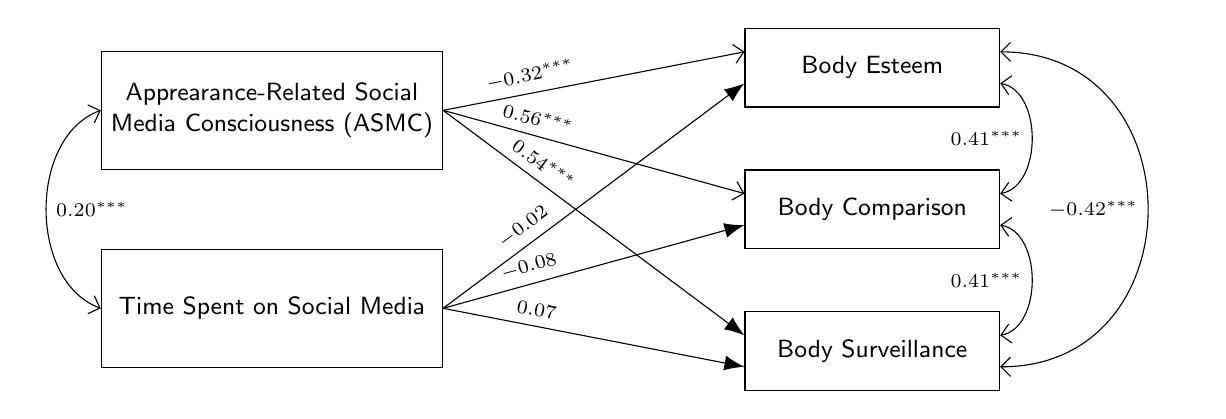
\begin{tikzpicture}
      \tikzset{rblock/.style={draw, font=\small\sffamily, text centered, 
        text width=30mm, minimum height = 10mm, node distance=1.8cm}};
      \tikzset{lblock/.style={draw, font=\small\sffamily, text centered, 
        text width=41mm, minimum height = 15mm, node distance=1.8cm}};
      \tikzset{arrows={[scale=1.5]}};
      \tikzset{label/.style={font=\scriptsize}};
      \node[rblock](bodyS) at (0,0){Body Surveillance};
      \node[rblock, above of = bodyS](bodyC) {Body Comparison}; 
      \node[rblock, above of = bodyC](bodyE) {Body Esteem}; 

      \coordinate[left = 6cm of bodyC] (lbpivot);
      \node[lblock, below = 5mm of lbpivot](TSSM){Time Spent on Social Media};
      \node[lblock, above = 5mm of lbpivot](ASMC){\mbox{Apprearance-Related} Social Media \mbox{Consciousness} (ASMC)};

      %TSSMからのパス
      \draw[label,-Latex] (TSSM.east)--node[pos=.3,above,sloped]{$0.07$}($(bodyS.west)+(0,-2mm)$) ;
      \draw[label,-Latex] (TSSM.east)--node[pos=.3,above,sloped]{$-0.08$}($(bodyC.west)+(0,-2mm)$);
      \draw[label,-Latex] (TSSM.east)--node[pos=.3,above,sloped]{$-0.02$}($(bodyE.west)+(0,-2mm)$);

      %ASMCからのパス
      \draw[label,-Latex] (ASMC.east)--node[pos=.3,above,sloped]{$0.54^{\scriptscriptstyle{***}}$}($(bodyS.west)+(0,+2mm)$);
      \draw[label,-Straight Barb] (ASMC.east)--node[pos=.3,above,sloped]{$0.56^{\scriptscriptstyle{***}}$}($(bodyC.west)+(0,+2mm)$);
      \draw[label,-Straight Barb] (ASMC.east)--node[pos=.3,above,sloped]{$-0.32^{\scriptscriptstyle{***}}$}($(bodyE.west)+(0,+2mm)$);

      % 左側の曲線
      \draw[label,Straight Barb-Straight Barb](TSSM.west) to [out = 160, in= 200] node[midway,right]{$0.20^{\scriptscriptstyle{***}}$} (ASMC.west);

      % 右内側の曲線
      \draw[label,Straight Barb-Straight Barb]($(bodyS.east)+(0,2mm)$) 
        to [out = 10, in= -10] node[midway,left]{$0.41^{\scriptscriptstyle{***}}$} ($(bodyC.east)+(0,-2mm)$);
      \draw[label,Straight Barb-Straight Barb]($(bodyC.east)+(0,2mm)$) 
        to [out = 10, in= -10] node[midway,left]{$0.41^{\scriptscriptstyle{***}}$} ($(bodyE.east)+(0,-2mm)$);

      % 右外側の曲線
      \draw[label,Straight Barb-Straight Barb]($(bodyS.east)+(0,-2mm)$)
        .. controls ($(bodyS.east)+(2.5cm,-2mm)$) and
        ($(bodyE.east)+(2.5cm,2mm)$) .. node[midway,left]{$-0.42^{\scriptscriptstyle{***}}$}($(bodyE.east)+(0,2mm)$);
    \end{tikzpicture}
    \note{The path analysis shows associations between ASMC and endogenous body-related variables (body esteem, body comparison, and body surveillance), controlling for time spent on social media. Coefficients presented are standardized linear regression coefficients. Adapted from APA Style: Sample Figures. https://apastyle.apa.org/style-grammar-guidelines/tables-figures/sample-figures}

    $^{\scriptscriptstyle{***}}p<.001$.
  \end{minipage}
\end{figure}

図の参照位置と挿入位置を別にしたい場合,図の参照はせず図の挿入位置のみを指定したい場合には,\texttt{\textbackslash{}fighere\{\}}コマンドを使用してください。本文中の図の挿入希望位置で\texttt{\textbackslash{}fighere\{2\}}と指定すると,その行の欄外に「Figure 2」の挿入指示マークが表示されます\fighere{2}。


\subsection{図の番号,図の題}

表のページでは,図の番号は(Figure 1,Figure 2など)の直後に改行し,題をつけることになっています。\texttt{jjpsy}クラスでは,この書式のとおりに表番号と題を作成します。なお,表の題の末尾にはピリオド(.)や句点(。)はつけませんが,本クラスファイルではこのチェックは行なっていません。また,2022年版の手びきから,図の番号と題は表と同様に図の上につけることになっているので注意が必要です。\texttt{\textbackslash{}includegraphics\{\}}などを用いて図を挿入する場合には,\texttt{\textbackslash{}caption\{\}}の後に行うようにしてください。


\subsection{図の注}

図全体に関する注は,figure環境内で\texttt{\textbackslash{}note\{\}}コマンドを使用することで作成できます。本文中の脚注に使用するコマンドと同じ名前ですが,figure環境内で図の後に\texttt{\textbackslash{}note\{\}}を使用した場合,その内容は図の下に「\emph{Note}.」(日本語環境では「注)」)つきで表示されます。

図の特定部分に関する注(\textsuperscript{a, b, c}や\textsuperscript{*, **}など)に関する説明は,\texttt{\textbackslash{}note\{\}}と\texttt{\textbackslash{}end\{table\}}の間に記載してください。

\section{文献の引用}

文献の引用を効率化するには,『心理学研究』の文献引用書式にそったBib\LaTeX{}用スタイルファイルである\texttt{biblatex-jpa}が便利です。\texttt{biblatex-jpa}を使用するには,\texttt{biblatex-jpa}の関連ファイル(jpa.bbx,jpa.cbx,jpa.dbx)を\LaTeX{}管理下のフォルダに置き,プリアンブルで「\texttt{\textbackslash{}usepackage[backend=biber,style=jpa]\{biblatex\}}」と指定してスタイルファイルを読み込みます。また,文献情報を記載した\texttt{.bib}ファイルを\texttt{\textbackslash{}addbibresource\{\}}で指定します。

本文中で\texttt{\textbackslash{}textcite\{\}}または\texttt{\textbackslash{}parencite\{\}}で文献を参照すると,その文献が書式にそって本文中に引用されます。また,文献の挿入位置(通常は考察の後ろ)で\texttt{\textbackslash{}printbibliography[title=引用文献]}として指定することにより,整形された文献リストが作成されます。\texttt{biblatex-jpa}の詳細については,\texttt{biblatex-jpa}のマニュアルを参照してください。

\section{まとめ}

\texttt{jjpsy}クラスは,『心理学研究』投稿用の原稿を作成する際の細々した設定をできるだけ自動化できるよう作成したものです。本クラスファイルが用意しているのは非常に基本的な機能のみですが,\LaTeX{}は非常に自由度の高い組版ツールです。足りない部分,気に入らない部分は,各自で設定を追加したり,変更したりしていけばよいでしょう。

% こに引用文献リストを作成
\printbibliography[title=引用文献]

% ここに脚注を表示
\noteshere 
\end{document}